\titlebox[nynorsk]

\Problem{($\SI{20}{\percent}$)}

A \emph{vertex cover} for a graph
$\Gamma = (V, E)$ is a collection 
of vertices that meets every edge. 
%
The graph in \cref{fig:MAT-2202-31-05-2017-problem-1}
%
\begin{figure}[H]\centering
    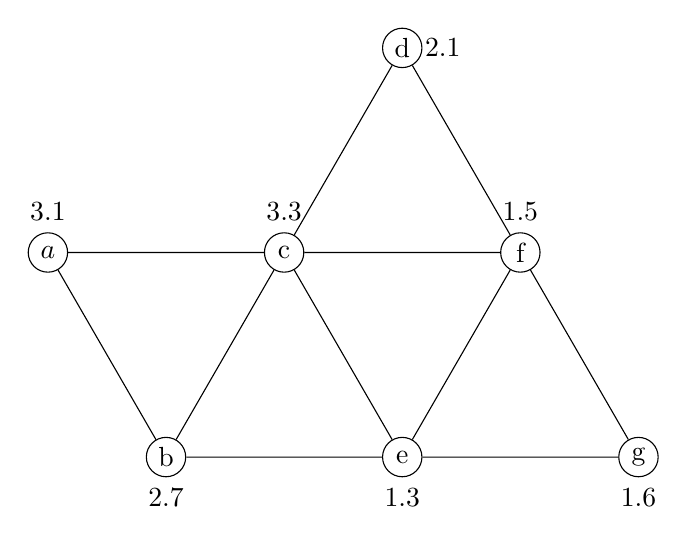
\begin{tikzpicture}[every node/.style={draw,circle,minimum size=5mm,inner sep=0}]
    \def\distance{3cm}
        \node[label=above:{$3.1$}] (a) at (0,0) {$a$};
        \path (a) ++(-60:\distance) 
              node[label=below:{$2.7$}] (b) {b}; 
        \path (a) ++(0:\distance)%
              node[label=above:{$3.3$}] (c) {c}; 
        \path (c) ++(60:\distance)%
              node[label=right:{$2.1$}] (d) {d};
        \path (c) ++(-60:\distance)%
              node[label=below:{$1.3$}] (e) {e};
        \path (c) ++(0:\distance)% 
              node[label=above:{$1.5$}] (f) {f};
        \path (f) ++(-60:\distance)%
              node[label=below:{$1.6$}] (g) {g};
        
    \draw (a) -- (c) -- (d) -- (f) -- (g) -- (e) -- (b) -- (a) (c) -- (b) (c) -- (f) -- (e) -- (c);
    \end{tikzpicture}
    \caption{}
    \label{fig:MAT-2202-31-05-2017-problem-1}
\end{figure}
%
has a weight function $\fun[w]{V}{\R^+}$ on the vertices.
The weights are marked in the sketch. The total weight of vertex cover is the sum of the weights of the vertices in the cover.

\begin{subproblem}
    For the graph in \cref{fig:MAT-2202-31-05-2017-problem-1} exhibit the steps of a greedy algorithm
    to obtain a vertex cover with small total weight.
\end{subproblem}

\begin{subproblem}
    For the graph in \cref{fig:MAT-2202-31-05-2017-problem-1}, formulate the problem of obtaining a vertex cover 
    with minimum total weight as an Integer Linear Programming problem.
\end{subproblem}

\newpageNotLF

\Problem{($\SI{30}{\percent}$)}

\begin{subproblem}
    Establish that the function
    %
    \begin{equation}
        f(x, y) = x^2 - 2xy + 7y^2 + \sin(x),
    \end{equation}
    %
    is strictly convex everywhere.
\end{subproblem}

\begin{subproblem}
    For the function $f$, compute the Newton step $\vp$ at
    $\vx_0 = \mat{0 & 0}\tran$. Is this Newton step a descent 
    direction?
\end{subproblem}

\begin{subproblem}
    Explain briefly how Newton's method applied to a strictly convex
    $C^2$ function may be modified so that it becomes a reliable downhill
    search. The proposed modification should ensure that full Newton
    steps are take when close to a minimum point.
\end{subproblem}


\Problem{($\SI{20}{\percent}$)}

\bgroup \newcommand{\dollar}[1]{$\$\,#1$}

A company plans to build six factories over the next
four years. It will build factories of a fixed size, at a cost that it has forecast
to vary somewhat over the years. The number of new factories justified by
projected demand, and the forecast cost to build a factory, are given in \cref{tab:MAT-2202-31-05-2017-problem-3}.
%
\begin{table}[H]
    \centering
    \caption{}
    \label{tab:MAT-2202-31-05-2017-problem-3}
    \begin{tabular}{c c c}
        \toprule
             Year & New factories at end of year & Cost per factory\\
        \midrule
             $0$ & $\leq 1$ & \dollar{32\text{m}} \\
             $1$ & $\leq 2$ & \dollar{32\text{m}} \\
             $2$ & $\leq 5$ & \dollar{32\text{m}} \\
             $3$ & $=6$ & \dollar{32\text{m}} \\
        \bottomrule
    \end{tabular}
\end{table}
%
A factory can be built within a single year, but no more than two can be built
in a year. During any year in which the company builds one or two factories, 
it incurs a lump-sum cost of \dollar{2\text{m}}. We ignore interest charges 
formulatea dynamic programming model to minimise the total cost of the capacity
expansion, but do not solve it.
\egroup

\newpageNotLF


\Problem{($\SI{30}{\percent}$)}

\begin{subproblem}
    The linear program
    %
    \begin{align*}
        \minus x + y & \to \min \\
           -   x + y & = 1 \\
               x , y & \geq 0,
    \end{align*}
    %
    is in standard form. Sketch the feasible set $S$ in a rectangular coordinate
    system, and mark off the basic solution(s), the basic feasible solution(s), and
    the optimal solution(s) in the sketch.
\end{subproblem}

\begin{subproblem}
    Show that if $\vx_1$ and $\vx_2$ are optimal solutions of an $LP$ problem, then
    $\vx_3 = \num{0.5}\vx_1 + \num{0.5}\vx_2$ is also an optimal solution of the same LP problem.
\end{subproblem}

\begin{subproblem}
    The LP problem
    %
    \begin{alignat*}{2}
                 3 x_1 -            x_2 - x_3 &&\longrightarrow &\min \\
        \phantom{2}x_1 + \phantom{2}x_2 + x_3 &&{} + s_1 \geq & \ 2 \\
                 2 x_1 +          5 x_2 + x_3 &&{} + s_2 \geq & \ 7 \\
                   x_1,             x_2,  x_3,s_1,e_2 && \geq & \ 0, 
    \end{alignat*}
    %
    is in standard form. The basic feasible solution
    %
    \begin{equation}
        \vx 
        = \mat{x_1 & x_2 & x_3 & s_1 & s_2}\tran 
        = \mat{  1 &   1 &   1 &   1 &   0}\tran,
    \end{equation}
    %
    is given. Perform a single step of the simplex method to obtain from 
    $\vx$ a new basic feasible solution that improves the objective.
\end{subproblem}